\documentclass[
11pt, % The default document font size, options: 10pt, 11pt, 12pt
codirector, % Uncomment to add a codirector to the title page
]{charter} 




% El títulos de la memoria, se usa en la carátula y se puede usar el cualquier lugar del documento con el comando \ttitle
%\titulo{Título del proyecto} 
\titulo{Dispositivo para pruebas de comunicación con satélites} 

% Nombre del posgrado, se usa en la carátula y se puede usar el cualquier lugar del documento con el comando \degreename
\posgrado{Carrera de Especialización en Sistemas Embebidos} 
%\posgrado{Carrera de Especialización en Internet de las Cosas} 
%\posgrado{Carrera de Especialización en Intelegencia Artificial}
%\posgrado{Maestría en Sistemas Embebidos} 
%\posgrado{Maestría en Internet de las cosas}

% Tu nombre, se puede usar el cualquier lugar del documento con el comando \authorname
\autor{Ing. Facundo G. Colavitte} 

% El nombre del director y co-director, se puede usar el cualquier lugar del documento con el comando \supname y \cosupname y \pertesupname y \pertecosupname
\director{Esp. Ing. Julián Bustamante Narvaez}
\pertenenciaDirector{FIUBA} 
% FIXME:NO IMPLEMENTADO EL CODIRECTOR ni su pertenencia
%\codirector{John Doe} % para que aparezca en la portada se debe descomentar la opción codirector en el documentclass
%\pertenenciaCoDirector{FIUBA}

% Nombre del cliente, quien va a aprobar los resultados del proyecto, se puede usar con el comando \clientename y \empclientename
\cliente{Ing. David Vilaseca}
\empresaCliente{Satellogic}

% Nombre y pertenencia de los jurados, se pueden usar el cualquier lugar del documento con el comando \jurunoname, \jurdosname y \jurtresname y \perteunoname, \pertedosname y \pertetresname.
\juradoUno{Nombre y Apellido (1)}
\pertenenciaJurUno{pertenencia (1)} 
\juradoDos{Nombre y Apellido (2)}
\pertenenciaJurDos{pertenencia (2)}
\juradoTres{Nombre y Apellido (3)}
\pertenenciaJurTres{pertenencia (3)}
 
\fechaINICIO{20 de octubre de 2022}		%Fecha de inicio de la cursada de GdP \fechaInicioName
\fechaFINALPlan{8 de diciembre de 2022} 	%Fecha de final de cursada de GdP
\fechaFINALTrabajo{21 de agosto de 2023}	%Fecha de defensa pública del trabajo final


\begin{document}

\maketitle
\thispagestyle{empty}
\pagebreak


\thispagestyle{empty}
{\setlength{\parskip}{0pt}
\tableofcontents{}
}
\pagebreak


\section*{Registros de cambios}
\label{sec:registro}


\begin{table}[ht]
\label{tab:registro}
\centering
\begin{tabularx}{\linewidth}{@{}|c|X|c|@{}}
\hline
\rowcolor[HTML]{C0C0C0} 
Revisión & \multicolumn{1}{c|}{\cellcolor[HTML]{C0C0C0}Detalles de los cambios realizados} & Fecha      \\ \hline
v0.0      & Creación del documento                                 &\fechaInicioName \\ \hline
v1.0      & Se completa hasta el punto 5 inclusive                 & 03 de noviembre de 2022 \\ \hline
v2.0      & Se completa hasta el punto 9 inclusive                & 10 de noviembre de 2022 \\ \hline
v3.0      & Se completa hasta el punto 12 inclusive               & 17 de noviembre de 2022 \\ \hline
%v4.0      & Se completa el plan	                               & 24 de noviembre de 2022 \\ \hline
\end{tabularx}
\end{table}

\pagebreak



\section*{Acta de constitución del proyecto}
\label{sec:acta}

\begin{flushright}
Buenos Aires, \fechaInicioName
\end{flushright}

\vspace{2cm}

Por medio de la presente se acuerda con el \authorname\hspace{1px} que su Trabajo Final de la \degreename\hspace{1px} se titulará ``\ttitle'', consistirá esencialmente en el diseño de un prototipo modular, versátil, para realizar pruebas de comunicación unidireccional con satélites de órbita baja usando un módulo LoRa, y tendrá un presupuesto preliminar estimado de 600 hs de trabajo y \$30.000, con fecha de inicio \fechaInicioName\hspace{1px} y fecha de presentación pública \fechaFinalName.

Se adjunta a esta acta la planificación inicial.

\vfill

% Esta parte se construye sola con la información que hayan cargado en el preámbulo del documento y no debe modificarla
\begin{table}[ht]
\centering
\begin{tabular}{ccc}
\begin{tabular}[c]{@{}c@{}}Ariel Lutenberg \\ Director posgrado FIUBA\end{tabular} & \hspace{2cm} & \begin{tabular}[c]{@{}c@{}}\clientename \\ \empclientename \end{tabular} \vspace{2.5cm} \\ 
\multicolumn{3}{c}{\begin{tabular}[c]{@{}c@{}} \supname \\ Director del Trabajo Final\end{tabular}} \vspace{2.5cm} \\
%\begin{tabular}[c]{@{}c@{}}\jurunoname \\ Jurado del Trabajo Final\end{tabular}     &  & \begin{tabular}[c]{@{}c@{}}\jurdosname\\ Jurado del Trabajo Final\end{tabular}  \vspace{2.5cm}  \\
%\multicolumn{3}{c}{\begin{tabular}[c]{@{}c@{}} \jurtresname\\ Jurado del Trabajo Final\end{tabular}} \vspace{.5cm}                                                                     
\end{tabular}
\end{table}




\section{1. Descripción técnica-conceptual del proyecto a realizar}
\label{sec:descripcion}

El siguiente proyecto tendrá como objetivo desarrollar un prototipo para realizar pruebas de comunicación unidireccional con satélites de la empresa Satellogic. Esta última posee actualmente satélites de órbita baja para mapeo de la superficie terrestre mediante sistema de capturas de imágenes. Su objetivo es agregar a su cartera de servicios satelitales la posibilidad de recibir información de dispositivos IoT en tierra para ofrecerle una alternativa económica a los medios de comunicación tradicionales. Para esto, se realizará un dispositivo modular, que permita cambiar fácilmente la antena de transmición, incorporar estapas de amplificación de señal y modificación y carga del firmware de forma simple por USB. Esto da como resultado un dispositivo versátil que permite enviar datos tomados en tierra y emitirlos a la frecuencia de comunicación de los satélite de Satellogic.

Durante el actual proyecto solo se realizará comunicación entre dispositivos en tierra, no una comunicación real con un satélite. Tras finalizar el proyecto, la empresa probará las comunicaciones con los satélites en órbita, quedando dicha prueba fuera del alcance del presente trabajo. La comunicación descrita previamente entre dispositivos IoT y satélites no existe hoy en día y Satelogic tiene la hipótesis de que la comunicación LoRa a 920 MHz podría funciona.
El dispositivo deberá emitir señal a través de un módulo LoRa de forma unidireccional. Los datos a enviar por el prototipo deben poder ser tomados por USB o Wi-Fi.


Como se observa en la figura \ref{fig:diagBloques}, el dispositivo posee:
\begin{itemize}
	\item Un puerto de conexión USB para comunicación con ordenadores locales.
	\item Conexión Wi-Fi para ser manejado de forma remota.
	\item Alimentación externa.
	\item Puerto de conexión para antena tipo QFH.
\end{itemize}

\begin{figure}[htpb]
\centering 
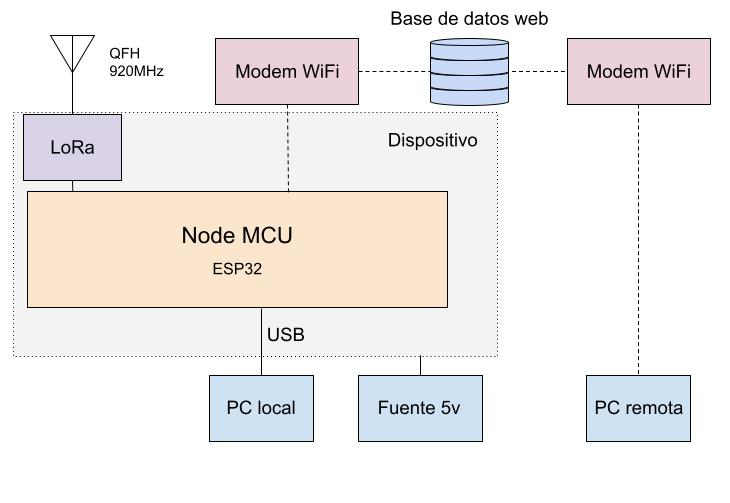
\includegraphics[width=.8\textwidth]{./Figuras/Diagrama de bloques.jpg}
\caption{Diagrama en bloques del sistema.}
\label{fig:diagBloques}
\end{figure}

\vspace{25px}

La propuesta de valor del proyecto es que a día de hoy no existe en el mercado un dispositivo comercial específico para tomar datos por USB y enviarlos a satélites de órbita baja de forma económica.
El desarrollo de este dispositivo se hará a través de dos trabajos de posgrado, uno es este, que se destaca en incorporar conexión Wi-Fi. Esto permite que el dispositivo pueda utilizarse de forma remota incluso cuando las condiciones climáticas no sean óptimas para el personal que lo comandará.

\section{2. Identificación y análisis de los interesados}
\label{sec:interesados}


\begin{table}[ht]
%\caption{Identificación de los interesados}
%\label{tab:interesados}
\begin{tabularx}{\linewidth}{@{}|l|X|X|l|@{}}
\hline
\rowcolor[HTML]{C0C0C0} 
Rol           & Nombre y Apellido & Organización 	& Puesto 	\\ \hline
Auspiciante   & \clientename      &\empclientename	& Director de Research 	\\ \hline
Cliente       & \clientename      &\empclientename	& Director de Research 	\\ \hline
Responsable   & \authorname       & FIUBA        	& Alumno 	\\ \hline
Colaboradores & Ing. Scasserra Marco   & FIUBA         	& Alumno   	\\ \hline
Orientador    & \supname	      & \pertesupname 	& Director Trabajo final \\ \hline
Usuario final & Ing. Pega Luciano      &\empclientename	& Ingeniero en Research  \\ \hline
\end{tabularx}
\end{table}


\begin{itemize}
	\item Pega Luciano: trabaja en la misma área que el cliente. Puede responder preguntas de requerimientos técnicos y validar el proyecto.
	\item Scasserra Marco: trabaja en un proyecto final del CESE de la misma temática para el mismo cliente.
	\item \supname: posee experiencia en módulos LoRa.
\end{itemize}



\section{3. Propósito del proyecto}
\label{sec:proposito}

El propósito del proyecto es diseñar un dispositivo que permita realizar pruebas de comunicación con satélites de órbita baja para una posterior implementación de dicha tecnología en dispositivos IoT. El prototípo debe ser versátil y estar conformado principalmente por módulos electrónicos comerciales para facilitar su posterior modificación según lo ameriten las pruebas.


\section{4. Alcance del proyecto}
\label{sec:alcance}

El proyecto incluye:
\begin{itemize}
	\item Un prototipo físico con el firmware cargado.
	\item Código fuente del firmware.
	\item Esquemático del hardware.
	\item Sistema de alimentación.
\end{itemize}
El proyecto no incluye:
\begin{itemize}
	\item Dispositivo comercial.
	\item Script que decodifica la señal IQ recibida en el satélite.
	\item Software de escritorio para envío de datos al dispositivo.
	\item Montaje del dispositivo.
\end{itemize}


\section{5. Supuestos del proyecto}
\label{sec:supuestos}

Para el desarrollo del presente proyecto se supone que:

\begin{itemize}
	\item Si dos dispositivos se pueden comunicar en tierra por medio de módulos LoRa la señal puede ser recibida por un satélite que esté dentro del alcance del conjunto módulo LoRa-Antena.
	\item Disponibilidad de todos los materiales necesarios para la construcción del prototípo por parte de la empresa Satellogic. Los mismos se detallarán en la Lista de materiales conforme se realice el proyecto.
	\item No se presentaran retenciones a importaciones de los materiales necesarios que dificulten su disponibilidad.
	\item Se dispondrá de al menos 80 horas mensuales en promedio para dedicar al proyecto.
	\item Los materiales necesarios para las pruebas y construcción de prototipos se dispondran en un tiempo no mayor a dos semanas tras solicitarlos.
\end{itemize}

\section{6. Requerimientos}
\label{sec:requerimientos}

\begin{enumerate}
	\item Requerimientos funcionales
		\begin{enumerate}
			\item Se debe poder cambiar la antena y agregar etapas de amplificación sin modificar la PCB.
			\item El dispositivo debe poseer un puerto de conexión incluido en la PCB para cargar el firmware sin necesidad de extraer el microcontrolador.
			\item El módulo LoRa debe ser un E22 900M30S de EBYTE según solicitud de la empresa.
			\item El dispositivo debe poder funcionar solo conectando perisféricos y fuentes de alimentación, sin requerir un proceso de configuración superior a cinco minutos para ponerlo en funcionamiento.
			\item El usuario debe poder enviar mensajes desde una computadora al prototipo por medio de un terminal serie por USB.
			\item El dispositivo debe tener alimentación propia ya sea con fuente externa o con baterías.
			\item El sistema deberá contar con comunicación Wi-Fi para acceder a la base de datos web.
			\item El dispositivo debe poder recibir datos por USB sin encriptar. Esto permite el uso de una interfaz serial genérica.
		\end{enumerate}
	\item Requerimientos de documentación
		\begin{enumerate}
			\item Se debe entregar al cliente un manual de usuario que describa el funcionamiento y la operación del prototipo.
			\item Se debe entregar al cliente la documentación del firmware desarrollado con un detalle o  explicación detallada de cada función desarrollada.
			\item Se debe realizar al menos un informe de avance dirigido al cliente previo a la finalización del proyecto.
		\end{enumerate}
	\item Requerimiento de testing
		\begin{enumerate}
			\item Se deberá testear comunicación USB.
			\item Se deberá testear comunicación Wi-Fi.
			\item Se deberá testear el acceso a la base de datos web de forma aislada.
			\item Se debe testear la comunicación LoRa con un dispositivo en tierra que reciba la señal que el prototipo emite. Para el testeo los dispositivos pueden estar a distancias inferiores a un metro y sin uso obligatorio de una antena.
		\end{enumerate}
\end{enumerate}

\section{7. Historias de usuarios (\textit{Product backlog})}
\label{sec:backlog}

A continuación se enunciarán las historias de usuarios y su ponderación (story points). La estimación de la ponderación se realizará por medio de la serie Fibonacci. Se evaluará dificultad, complejidad y riesgo. Los pesos en la evaluación corresponderán a 0 para bajo y 8 para alto. El pseo final será el valor de la suma de las tres características mencionadas. En caso de que la suma no sea igual a un número de la secuencia de Fibonacci se le asignará a la historia el valor próximo superior.

\begin{enumerate}
	\item “Como usuario, quiero que el dispositivo sea compacto, robusto y ligero, de modo de poder llevarlo al lugar donde debe realizarse el experimento.”
		\begin{itemize}
		\item Dificultad: media/baja (3). Implica realizar un dimensionamiento de la batería y selección de la envolvente plástica.
		\item Complejidad: media (5). Se requiere realizar un diseño para la envolvente plásica con una protección IP32 o superior. El dispositivo debe contar con suficiente capacidad de batería para una hora de autonomía.
		\item riesgo: media/baja (3). El equipo debe estar cubierto de la lluvia de forma directa, en caso contrario la envolvente deberá tener un grado de protección IP65 o superior.
		\item Story point: 13.
		\end{itemize}
\vspace{5mm}
	\item “Como usuario, quiero que el dispositivo se conecte a Wi-Fi para poder operarlo de manera remota.“
		\begin{itemize}
		\item Dificultad: alta (8). Implica gran cantidad de horas para realizar una base de datos web y la programación de la comunicación Wi-Fi, interconexión con la base de datos y procesamiento de los datos recibidos por JSON.
		\item Complejidad: media (5). La comunicación con la base de datos por medio de Wi-Fi y procesamiento de los archivos json implica una dificultad media.
		\item riesgo: media (5). Existe el riesgo de que no se tenga una potencia de señal Wi-Fi suficiente en la ubicación en la que se desea colocar el dispositivo.
		\item Story point: 21.
		\end{itemize}
		
\vspace{5mm}
		
	\item “Como usuario, quiero que la interfaz de comunicación sea a través de una interfaz de linea de comando (CLI), para que la operación sea ágil.”
		\begin{itemize}
		\item Dificultad: media (5). Se requiere realizar funcionalidades que analicen la recepción por UART para diferenciar un comando a ejecutar de un simple texto a enviar por LoRa.
		\item Complejidad: media/baja (3). Se requiere una comunicacion UART con conversión a USB. El circuito integrado que realiza dicha tarea está incluido en el módulo Node-MCU.
		\item riesgo: bajo (1). No se presentan riesgos.
		\item Story point: 13.
		\end{itemize}
				
\vspace{5mm}
	
	\item “Como usuario, quiero que el dispositivo cuente con un conector de radio frecuencia (RF), de modo de poder elegir distintos tipos de antenas, o incluso agregar una etapa de amplificación adicional, de ser necesario.”
		\begin{itemize}
		\item Dificultad: media/baja (3). Se debe buscar el foot print del conector que mejor se adapte a las antenas que solicita Satellogic.
		\item Complejidad: baja (1). Se debe agregar el foot print del conector en el diseño de la PCB.
		\item riesgo: medio/bajo (3). En caso de utilizarse antenas con conector no compatible se debe adaptar la antena al prototipo.
		\item Story point: 8.
		\end{itemize}
				
\vspace{5mm}
	
	\item “Como usuario, quiero que el dispositivo sea suficientemente pequeño como para poder integrarse en un gabinete estanco, lo cual permitiría la operación en intemperie.”
		\begin{itemize}
		\item Dificultad: baja (1). Se debe buscar un gabinete estanco comercial apto para las medidas del prototipo.
		\item Complejidad: baja (1). No presenta complejidad.
		\item riesgo: medio/bajo (3). En caso de que se desee que el dispositivo cuente con terminales para realizar conecciones por fuera del gabinete, las mismas deben ser aptas para exterior.
		\item Story point: 5.
		\end{itemize}
\end{enumerate}


\section{8. Entregables principales del proyecto}
\label{sec:entregables}

Los entregables del proyecto son:
\begin{itemize}
	\item Manual de usuario del dispositivo.
	\item Diagrama esquemático del circuito.
	\item Código fuente.
	\item Lista de componentes electrónicos.
	\item Un prototipo funcional.
\end{itemize}



\section{9. Desglose del trabajo en tareas}
\label{sec:wbs}

\begin{enumerate}
\item Recopilación general de información sobre el proyecto (60 hs)
	\begin{enumerate}
	\item Investigar sobre tecnología Wi-Fi. (10 hs)
	\item Investigar sobre tecnología LoRa. (20 hs)
	\item Investigación específica sobre módulo LoRa E22. (10 hs)
	\item Investigar sobre antenas QFH. (10 hs)
	\item Investigar sobre base de datos web. (10 hs)
	\end{enumerate}
\item Planificación del proyecto (40 hs)
	\begin{enumerate}
	\item Realizar planificación del proyecto. (40 hs)
	\end{enumerate}
\item Hardware (120 hs)
	\begin{enumerate}
	\item Diseño del circuito esquemático. (25 hs)
	\item Cálculo de sistema de almacenamiento de energía. (20 hs)
	\item Selección de componentes. (15 hs)
	\item Diseño del PCB. (30 hs)
	\item Fabricación y ensamblado del PCB. (30 hs)
	\end{enumerate}
\item Firmware (120 hs)
	\begin{enumerate}
	\item Desarrollo de arquitectura del firmware. (20 hs)
	\item Diseño y programación de la máquina de estados finitos. (20 hs)
	\item Diseño y programación de comunicación LoRa. (10 hs)
	\item Diseño y programación de comunicación UART. (10 hs)
	\item Diseño y programación de comunicación Wi-Fi y base de datos. (40 hs)
	\item Configuración de la base de datos. (10 hs)
	\item Integración de las partes del firmware. (10 hs)
	\end{enumerate}
\item Pruebas (70 hs)
	\begin{enumerate}
	\item Pruebas y validación del hardware. (20 hs)
	\item Desarrollo de pruebas para el firmware. (30 hs)
	\item Verificación y validación del firmware. (20 hs)
	\end{enumerate}
\item Gabinete (50 hs)
	\begin{enumerate}
	\item Selección del gabinete. (10 hs)
	\item Montaje del prototipo en gabinete. (40 hs)
	\end{enumerate}
\item Procesos finales (140 hs)
	\begin{enumerate}
	\item Elaboración del informe de avance. (30 hs)
	\item Evaluación de requerimientos. (30 hs)
	\item Elaboración de la memoria del proyecto. (40 hs)
	\item Preparación de la presentación final. (40 hs)
	\end{enumerate}
\end{enumerate}


Cantidad total de horas: 600 hs.

\section{10. Diagrama de Activity On Node}
\label{sec:AoN}

A continuación se observa el gráfico del Activity on Node. Se señala en color rojo el camino crítico.
Los colores están asignados por categoría según el desgloce de tareas del inciso previo. Los tiempos t están dados en horas.

\begin{figure}[htpb]
\centering 
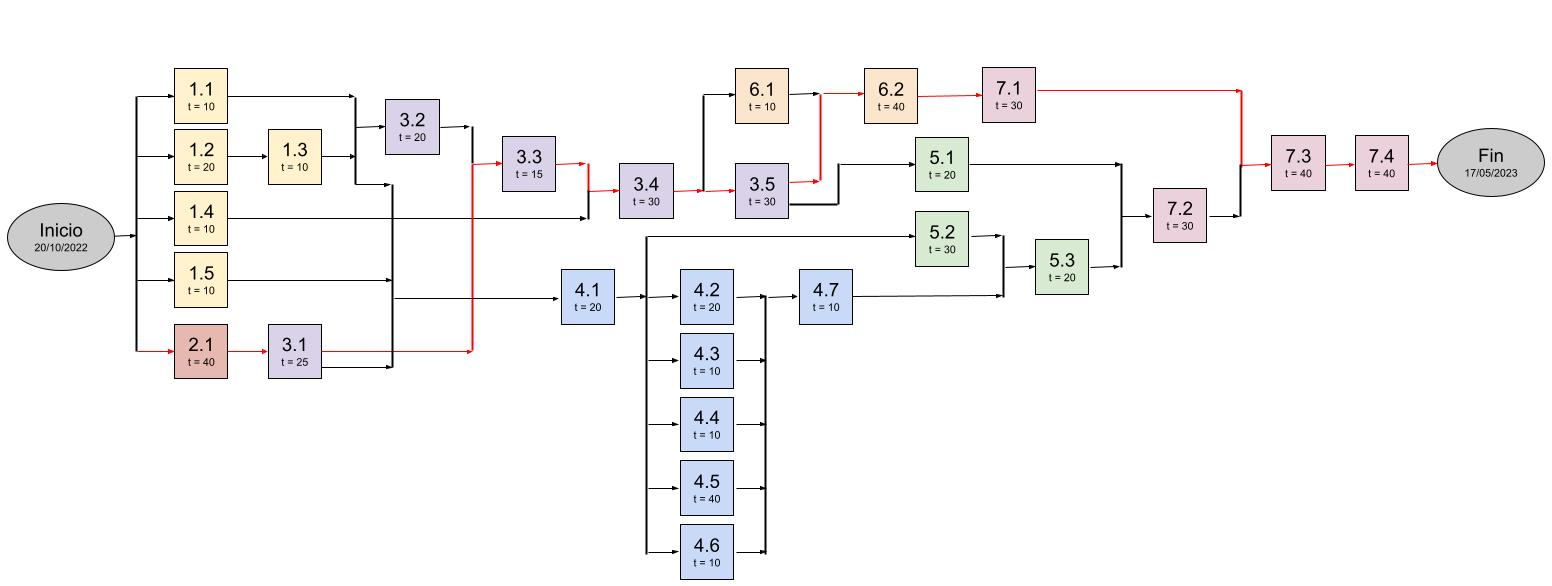
\includegraphics[width=1.08\textwidth]{./Figuras/Activity On Node.jpg}
\caption{Diagrama en \textit{Activity on Node}}
\label{fig:AoN}
\end{figure}


\section{11. Diagrama de Gantt}
\label{sec:gantt}
En la siguiente tabla se observa la lista de tareas, sus tiempos de duración, plazos de inicio y finalización. Cabe destacar que los tiempos asignados son en caso de poder realizar más de una tarea en simultaneo.

\begin{figure}[htpb]
\centering 
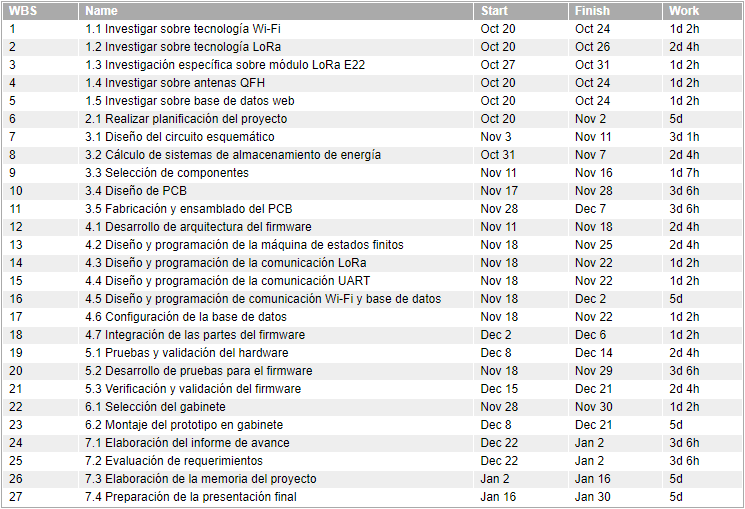
\includegraphics[width=1\textwidth]{./Figuras/Tabla Gantt.png}
\caption{Tabla del diagrama de Gantt.}
\label{fig:tablaGantt}
\end{figure}

\begin{landscape}
\begin{figure}[htpb]
\centering 
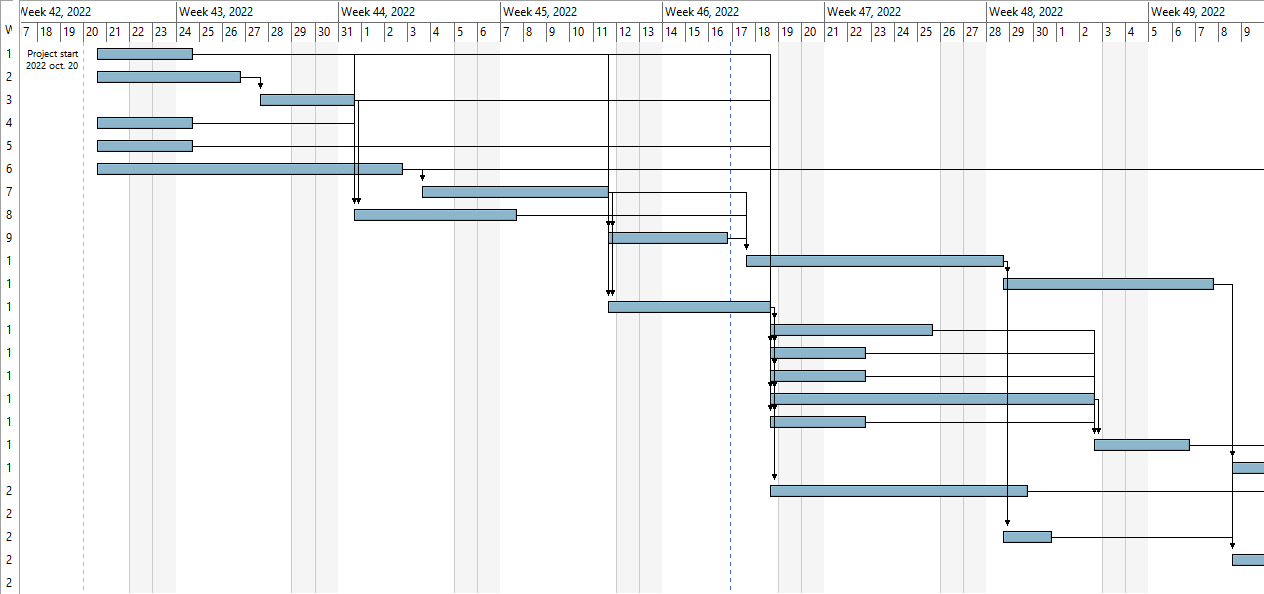
\includegraphics[height=.7\textheight]{./Figuras/Diagrama Gantt 1.png}
\caption{Diagrama de Gantt del proyecto, parte 1.}
\label{fig:diagGantt1}
\end{figure}
\end{landscape}

\begin{landscape}
\begin{figure}[htpb]
\centering 
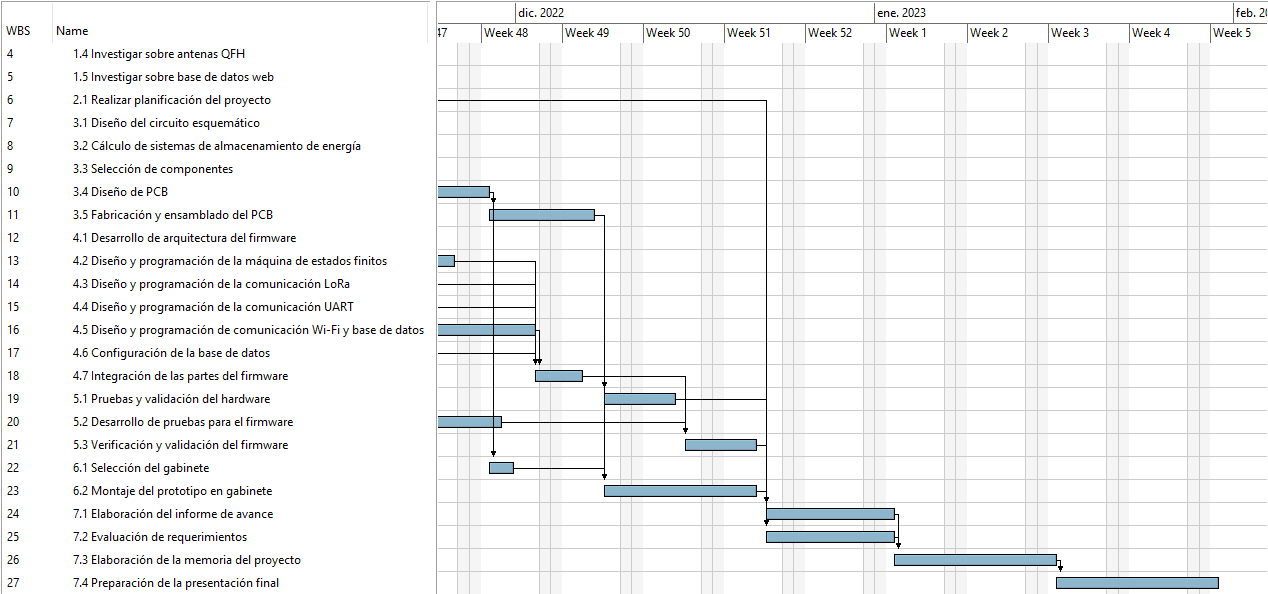
\includegraphics[height=.7\textheight]{./Figuras/Diagrama Gantt 2.png}
\caption{Diagrama de Gantt del proyecto, parte 2.}
\label{fig:diagGantt2}
\end{figure}
\end{landscape}

\begin{landscape}
Si se observa únicamente las interdependencias, las tareas pueden realizarse simultaneamente como se describe en los gráficos previos. Este no será el caso del presente proyecto, ya que el trabajo a realizar lo llevará a cabo una única persona. A continuación se muestra el diagramma de Gannt ordenado de forma tal de realizar una sola tarea a la vez.

\begin{figure}[htpb]
\centering 
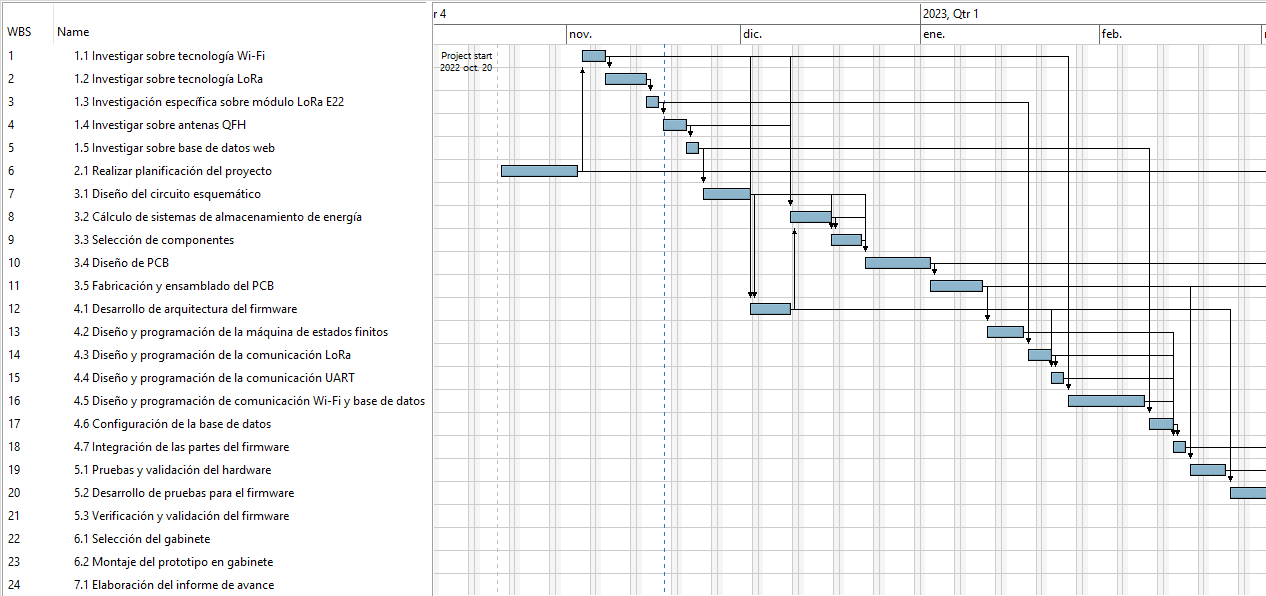
\includegraphics[height=.7\textheight]{./Figuras/Diagrama Gantt sin tareas en paralelo 1.png}
\caption{Diagrama de Gantt a seguir, parte 1.}
\label{fig:diagGantt3}
\end{figure}
\end{landscape}

\begin{landscape}
\begin{figure}[htpb]
\centering 
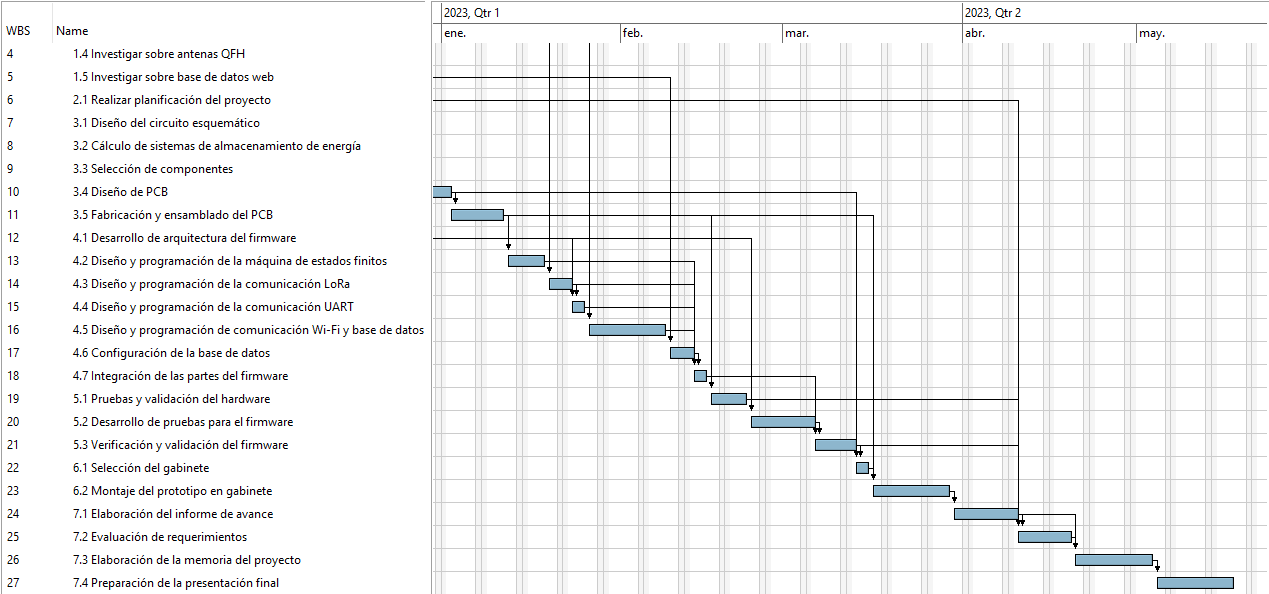
\includegraphics[height=.7\textheight]{./Figuras/Diagrama Gantt sin tareas en paralelo 2.png}
\caption{Diagrama de Gantt a seguir, parte 2.}
\label{fig:diagGantt4}
\end{figure}
\end{landscape}


\section{12. Presupuesto detallado del proyecto}
\label{sec:presupuesto}


\begin{table}[htpb]
\centering
\begin{tabularx}{\linewidth}{@{}|X|c|r|r|@{}}
\hline
\rowcolor[HTML]{C0C0C0} 
\multicolumn{4}{|c|}{\cellcolor[HTML]{C0C0C0}COSTOS DIRECTOS} \\ \hline
\rowcolor[HTML]{C0C0C0} 
Descripción &
  \multicolumn{1}{|c|}{\cellcolor[HTML]{C0C0C0}Cantidad} &
  \multicolumn{1}{c|}{\cellcolor[HTML]{C0C0C0}Valor unitario} &
  \multicolumn{1}{c|}{\cellcolor[HTML]{C0C0C0}Valor total} \\ \hline
  
\multicolumn{1}{|l|}{Placa Node-MCU (ESP32)} &1
   &\$ 4500
   &\$ 4500
   \\ \hline
\multicolumn{1}{|l|}{Módulo LoRa E22} &1
   &\$ 1600
   &\$ 1600
   \\ \hline
\multicolumn{1}{|l|}{Antena QFH 920 MHz} &1
   &\$ 2000
   &\$ 2000
   \\ \hline
\multicolumn{1}{|l|}{Batería LiPo} &1
   &\$ 4000
   &\$ 4000
   \\ \hline
\multicolumn{1}{|l|}{Caja estanca} &1
   &\$ 600
   &\$ 600
   \\ \hline
\multicolumn{1}{|l|}{Componentes electrónicos} &1
   &\$ 3000
   &\$ 3000
   \\ \hline
\multicolumn{3}{|c|}{SUBTOTAL} &
  \multicolumn{1}{c|}{\$ 15700} \\ \hline
\rowcolor[HTML]{C0C0C0} 
\multicolumn{4}{|c|}{\cellcolor[HTML]{C0C0C0}COSTOS INDIRECTOS} \\ \hline
\rowcolor[HTML]{C0C0C0} 
Descripción &
  \multicolumn{1}{c|}{\cellcolor[HTML]{C0C0C0}Cantidad} &
  \multicolumn{1}{c|}{\cellcolor[HTML]{C0C0C0}Valor unitario} &
  \multicolumn{1}{c|}{\cellcolor[HTML]{C0C0C0}Valor total} \\ \hline
\multicolumn{1}{|l|}{20\% del costo directo} &1
   &\$ 3140
   &\$ 3140
   \\ \hline
\multicolumn{1}{|l|}{Impuestos de importación del módulo LoRa 65\%} &1
   &\$ 1040
   &\$ 1040
   \\ \hline
\multicolumn{1}{|l|}{Envío de materiales} &1
   &\$ 3000
   &\$ 3000
   \\ \hline
\multicolumn{3}{|c|}{SUBTOTAL} &
  \multicolumn{1}{c|}{\$ 7180} \\ \hline
\rowcolor[HTML]{C0C0C0}
\multicolumn{3}{|c|}{TOTAL} &\$ 22880
   \\ \hline
\end{tabularx}%
\end{table}


\section{13. Gestión de riesgos}
\label{sec:riesgos}

\begin{consigna}{red}
a) Identificación de los riesgos (al menos cinco) y estimación de sus consecuencias:
 
Riesgo 1: detallar el riesgo (riesgo es algo que si ocurre altera los planes previstos de forma negativa)
\begin{itemize}
	\item Severidad (S): mientras más severo, más alto es el número (usar números del 1 al 10).\\
	Justificar el motivo por el cual se asigna determinado número de severidad (S).
	\item Probabilidad de ocurrencia (O): mientras más probable, más alto es el número (usar del 1 al 10).\\
	Justificar el motivo por el cual se asigna determinado número de (O). 
\end{itemize}   

Riesgo 2:
\begin{itemize}
	\item Severidad (S): 
	\item Ocurrencia (O):
\end{itemize}

Riesgo 3:
\begin{itemize}
	\item Severidad (S): 
	\item Ocurrencia (O):
\end{itemize}


b) Tabla de gestión de riesgos:      (El RPN se calcula como RPN=SxO)

\begin{table}[htpb]
\centering
\begin{tabularx}{\linewidth}{@{}|X|c|c|c|c|c|c|@{}}
\hline
\rowcolor[HTML]{C0C0C0} 
Riesgo & S & O & RPN & S* & O* & RPN* \\ \hline
       &   &   &     &    &    &      \\ \hline
       &   &   &     &    &    &      \\ \hline
       &   &   &     &    &    &      \\ \hline
       &   &   &     &    &    &      \\ \hline
       &   &   &     &    &    &      \\ \hline
\end{tabularx}%
\end{table}

Criterio adoptado: 
Se tomarán medidas de mitigación en los riesgos cuyos números de RPN sean mayores a...

Nota: los valores marcados con (*) en la tabla corresponden luego de haber aplicado la mitigación.

c) Plan de mitigación de los riesgos que originalmente excedían el RPN máximo establecido:
 
Riesgo 1: plan de mitigación (si por el RPN fuera necesario elaborar un plan de mitigación).
  Nueva asignación de S y O, con su respectiva justificación:
  - Severidad (S): mientras más severo, más alto es el número (usar números del 1 al 10).
          Justificar el motivo por el cual se asigna determinado número de severidad (S).
  - Probabilidad de ocurrencia (O): mientras más probable, más alto es el número (usar del 1 al 10).
          Justificar el motivo por el cual se asigna determinado número de (O).

Riesgo 2: plan de mitigación (si por el RPN fuera necesario elaborar un plan de mitigación).
 
Riesgo 3: plan de mitigación (si por el RPN fuera necesario elaborar un plan de mitigación).

\end{consigna}


\section{14. Gestión de la calidad}
\label{sec:calidad}

\begin{consigna}{red}
Para cada uno de los requerimientos del proyecto indique:
\begin{itemize} 
\item Req \#1: copiar acá el requerimiento.

\begin{itemize}
	\item Verificación para confirmar si se cumplió con lo requerido antes de mostrar el sistema al cliente. Detallar 
	\item Validación con el cliente para confirmar que está de acuerdo en que se cumplió con lo requerido. Detallar  
\end{itemize}

\end{itemize}

Tener en cuenta que en este contexto se pueden mencionar simulaciones, cálculos, revisión de hojas de datos, consulta con expertos, mediciones, etc.  Las acciones de verificación suelen considerar al entregable como ``caja blanca'', es decir se conoce en profundidad su funcionamiento interno.  En cambio, las acciones de validación suelen considerar al entregable como ``caja negra'', es decir, que no se conocen los detalles de su funcionamiento interno.

\end{consigna}

\section{15. Procesos de cierre}    
\label{sec:cierre}

\begin{consigna}{red}
Establecer las pautas de trabajo para realizar una reunión final de evaluación del proyecto, tal que contemple las siguientes actividades:

\begin{itemize}
	\item Pautas de trabajo que se seguirán para analizar si se respetó el Plan de Proyecto original:
	 - Indicar quién se ocupará de hacer esto y cuál será el procedimiento a aplicar. 
	\item Identificación de las técnicas y procedimientos útiles e inútiles que se emplearon, y los problemas que surgieron y cómo se solucionaron:
	 - Indicar quién se ocupará de hacer esto y cuál será el procedimiento para dejar registro.
	\item Indicar quién organizará el acto de agradecimiento a todos los interesados, y en especial al equipo de trabajo y colaboradores:
	  - Indicar esto y quién financiará los gastos correspondientes.
\end{itemize}

\end{consigna}


\end{document}
